\chapter{Model Interpretation} \label{chapter7}
Interpretability is crucial for medical use models. Clinical staff need to understand the way the model works in order to trust its prediction and compare it with their clinical judgment. Visualizations of the areas driving the classification can offer insights to clinicians (for example, highlighting very small lesions that could be missed) or be used as a pedagogical tool for learning clinicians. 

Interpretability techniques can also offer some guarantee against models misbehavior: for example, they may allow a clinician to identify a graphical artifact distorting classifications, as a reflection, which can make diagnosis more accurate and detect conditions of failure that can be improved. 

This chapter explores several techniques, both model specific and model agnostic, that we have implemented to explain the model previously introduced. We have tried to introduce these techniques in their context, discussing its theoretical justification and also exploring how they can help to approach lateral problems.

\section{Class activation maps}
Class activation maps are one of the preferred ways to visualize convolutional neural networks \cite{selvaraju2020grad-cam, jung2021explanations, bolei2016learning}. Suppose the last convolutional layer of the model outputs \( K \) feature maps \( A^k \in \mathbb{R}^{W \times H} \) indexed by \( i,j \).

These feature maps are then spatially pooled using Global Average Pooling and multiplied by the class weights to obtain the unnormalized probability of class \( c \):
\[
    Y^c = \sum_k w_k^c \frac{1}{Z} \sum_{i, j} A^k_{ij}
\]
where \( Z = WH \) is a normalization factor,

Since all operations involved are linear, this process is equivalent to calculating:
\[ 
    Y^c = \frac{1}{Z} \sum_{i, j} \sum_{k} w^k A^k_{ij} 
\]
but this version  includes the term \( H_{ij} = \sum_{k} w^c_k A^k_{ij} \), which expresses the result of the interaction between \( \bm{w}^c \) and \( A_{ij} \): the contribution of each part of the hidden representation to the output of \( Y^c \). We can translate this representation to an image and superimpose this term over the original input to understand which parts of the input drive the output of the model for class \( c \).

The graphic so obtained is called the \textit{class activation map} (CAM). If we fix \( c \) as the predicted class, then the CAM represents which parts of the image are the main responsible for the predicted output.

\begin{figure}[tb]
     \begin{subfigure}[b]{0.49\textwidth}
         \centering
         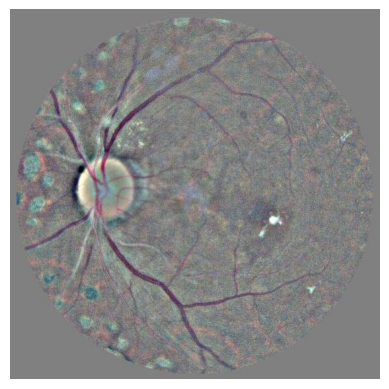
\includegraphics[width=0.49\textwidth,height=0.49\textwidth]{figures/chapter6/heatmaps/28699_left.png}
         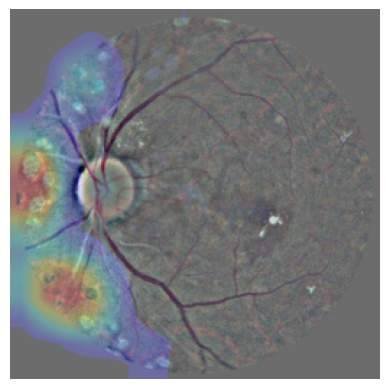
\includegraphics[width=0.49\textwidth,height=0.49\textwidth]{figures/chapter6/heatmaps/28699_left_heatmap.png}
         \caption{Predicted label: 4. Target: 4.}
    \end{subfigure}
    \hfill
    \begin{subfigure}[b]{0.49\textwidth}
         \centering
         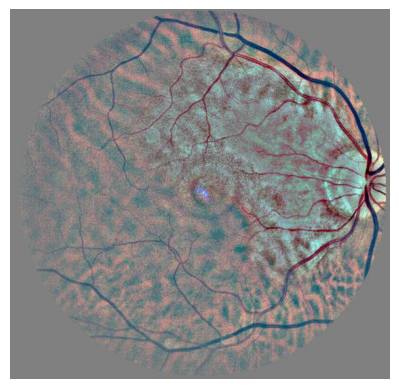
\includegraphics[width=0.49\textwidth,height=0.49\textwidth]{figures/chapter6/heatmaps/5_right.png}
         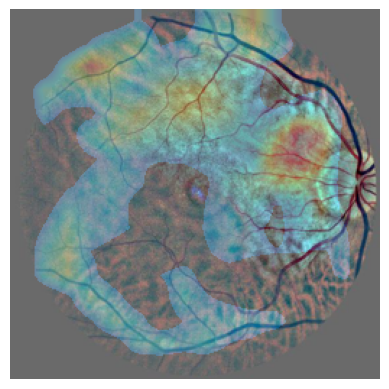
\includegraphics[width=0.49\textwidth,height=0.49\textwidth]{figures/chapter6/heatmaps/5_right_heatmap.png}
         \caption{Predicted label: 0. Target: 0.}
     \end{subfigure}

    \bigskip
    \begin{subfigure}[b]{0.49\textwidth}
         \centering
         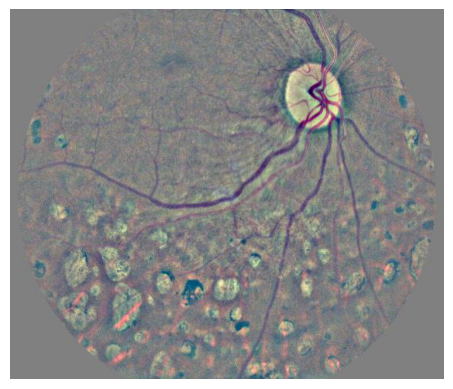
\includegraphics[width=0.49\textwidth,height=0.49\textwidth]{figures/chapter6/heatmaps/43670_left.png}
         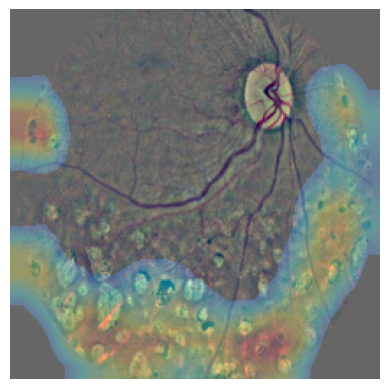
\includegraphics[width=0.49\textwidth,height=0.49\textwidth]{figures/chapter6/heatmaps/43670_left_heatmap.png}
        \caption{Predicted label: 4. Target: 4.}

    \end{subfigure}
    \hfill
    \begin{subfigure}[b]{0.49\textwidth}
         \centering
         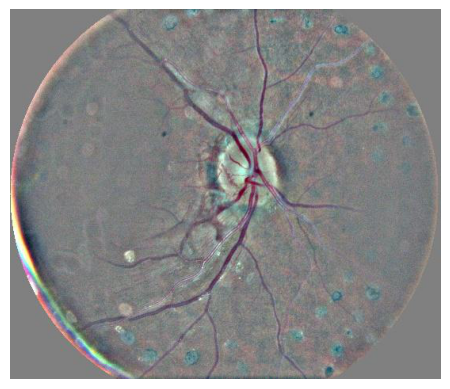
\includegraphics[width=0.49\textwidth,height=0.49\textwidth]{figures/chapter6/heatmaps/43716_left.png}
        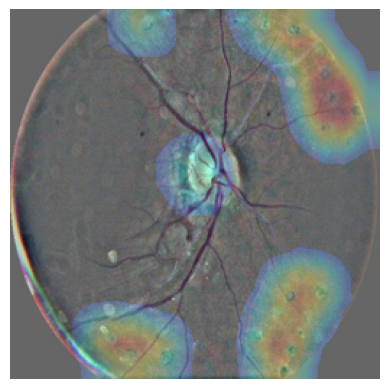
\includegraphics[width=0.49\textwidth,height=0.49\textwidth]{figures/chapter6/heatmaps/43716_left_heatmap.png}
        \caption{Predicted label: 4. Target: 4.}

     \end{subfigure}
     \centering
     \caption{Preprocessed images and class activation maps. To create the visualization we discard the bottom-50\% of the elements of the map and overlap it as pseudo-color.}
     \label{fig:heatmap}
\end{figure}

\Cref{fig:heatmap} shows both the preprocessed images and the result after overlapping the class activation map. In order to improve the readability of the result, we only preserved the top 20\% values of the CAM.

The images clearly show that the model successfully recognizes some lesions and its diagnostic importance. The map has a more disperse structures for those images with low or no DR affectation which is consistent with expectations, as these stages are characterized precisely by the absence of lesions.

There are two main problems with this approach, both related to the fact that the dimensions \( W, H \) is usually quite small (in this case, \( W = H = 16 \)). Because of repeated convolutions and pooling, each component \( H_{ij} \) summarizes information from a relatively large part of the image (a \( 32 \times 32 \) square in this case) and class activation maps won't be able to distinguish between the relative importance of objects contained in each of these patches. The second problem, is that to superimpose the map over the image we will need to resize it, usually using some kind of interpolation; this is a noisy process prone to include artifacts that may affect the analysis.

\subsection{Grad-CAM and related visualizations}
When presenting CAM we heavily relied on the fact that the CNN is structured as a convolutional block, followed by a global activation pooling and a single-layer classifier. However, not all models have this structure and a vector \( w^c \) for each class may not exist. We now explore a generalization that does not pose such a heavy requirement on the model architecture: Grad-CAM.

Let \( F^k \) be the global averaged pooled output:
\[
    F^k = \frac{1}{Z} \sum_{i, j} A^k_{ij}
\]
In the previous setting we had:
\[
    Y^c = \sum_k w_k^c F^k
\]
and using basic properties of gradients we can rewrite:
\[
    w_k^c = \sum_{i,j} \frac{\partial Y^c}{\partial A_{ij}^c}
\]
where the right-hand side is independent of the architecture of the network. This leads us to a generalization of CAM where the weights \( w_k^c \) have been substituted by \( \sum_{i,j} \frac{\partial Y^c}{\partial A_{ij}^c} \), an expression of the gradients.

A great number of variations and improvements have been built over this basis. \Cref{fig:visualizations} shows some related visualization over the same image: guided Grad-CAM, an anchor map and saliency diagram, obtained using an adaptation of a Python library \cite{journeyvisualization}.

\begin{figure}[htb]
     \begin{subfigure}[b]{0.24\textwidth}
         \centering
         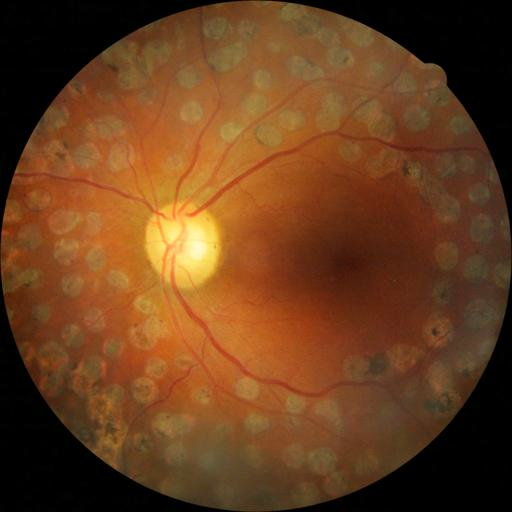
\includegraphics[width=\textwidth,height=\textwidth]{figures/chapter6/others/1707_left.jpeg}
         \caption{Original}
    \end{subfigure}
    \hfill
    \begin{subfigure}[b]{0.24\textwidth}
         \centering
         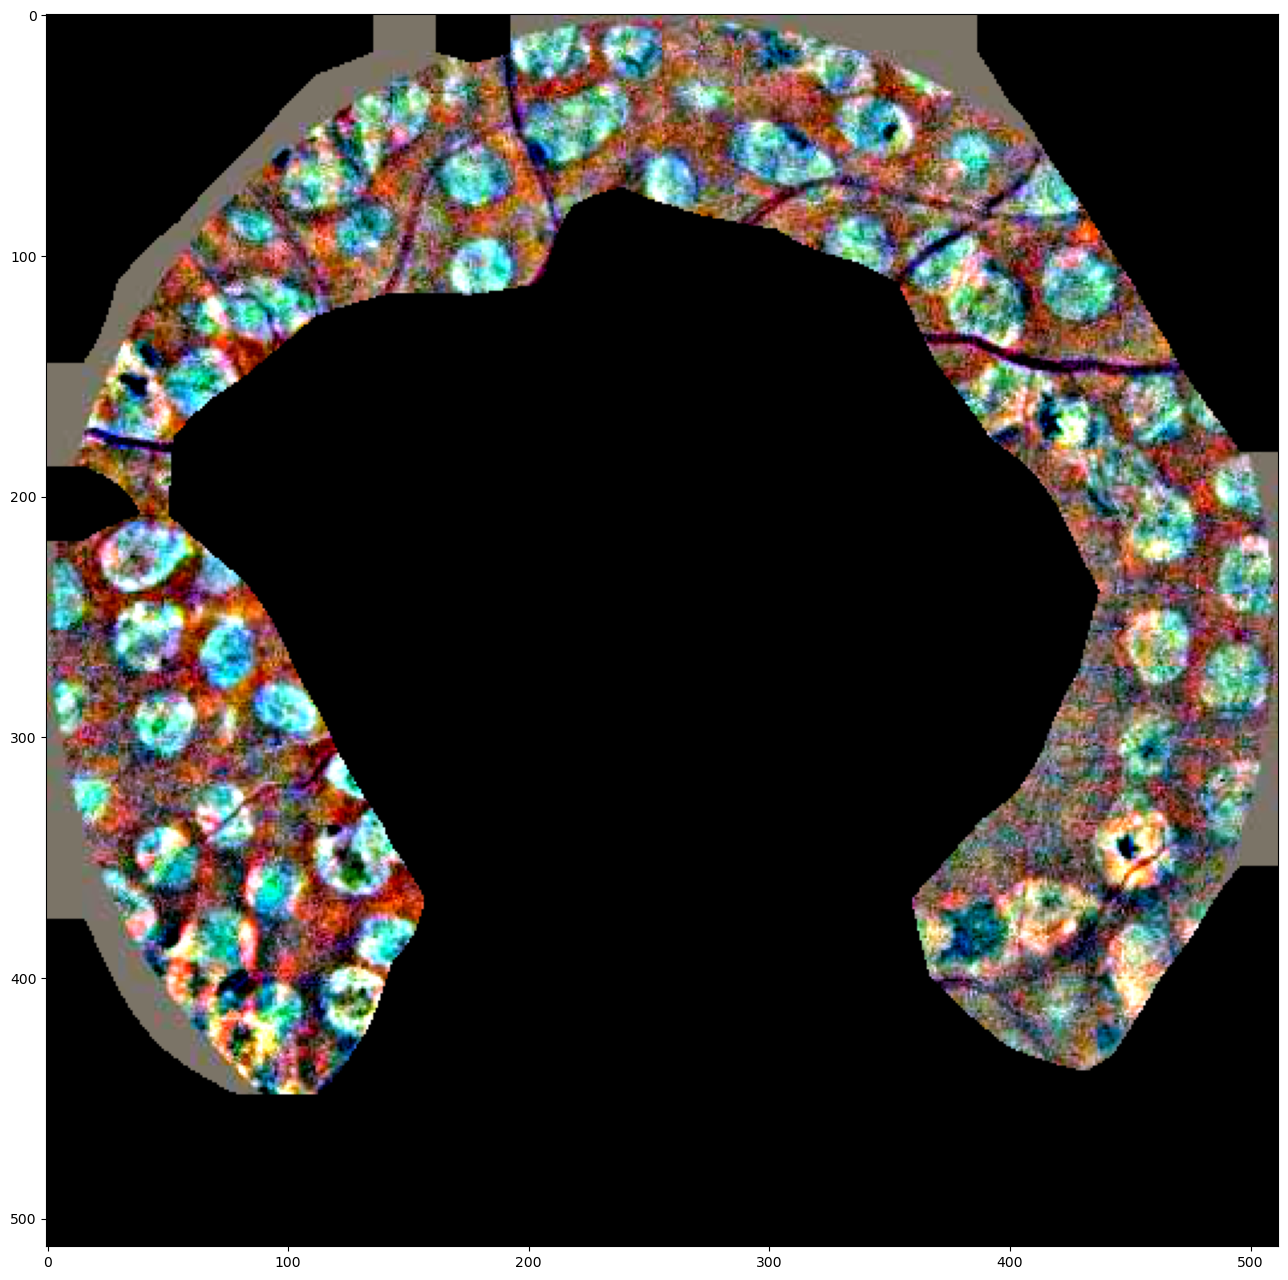
\includegraphics[width=\textwidth,height=\textwidth]{figures/chapter6/others/anchor.png}
         \caption{Anchor}
         \label{fig:anchor}
    \end{subfigure}
    \hfill
    \begin{subfigure}[b]{0.24\textwidth}
         \centering
         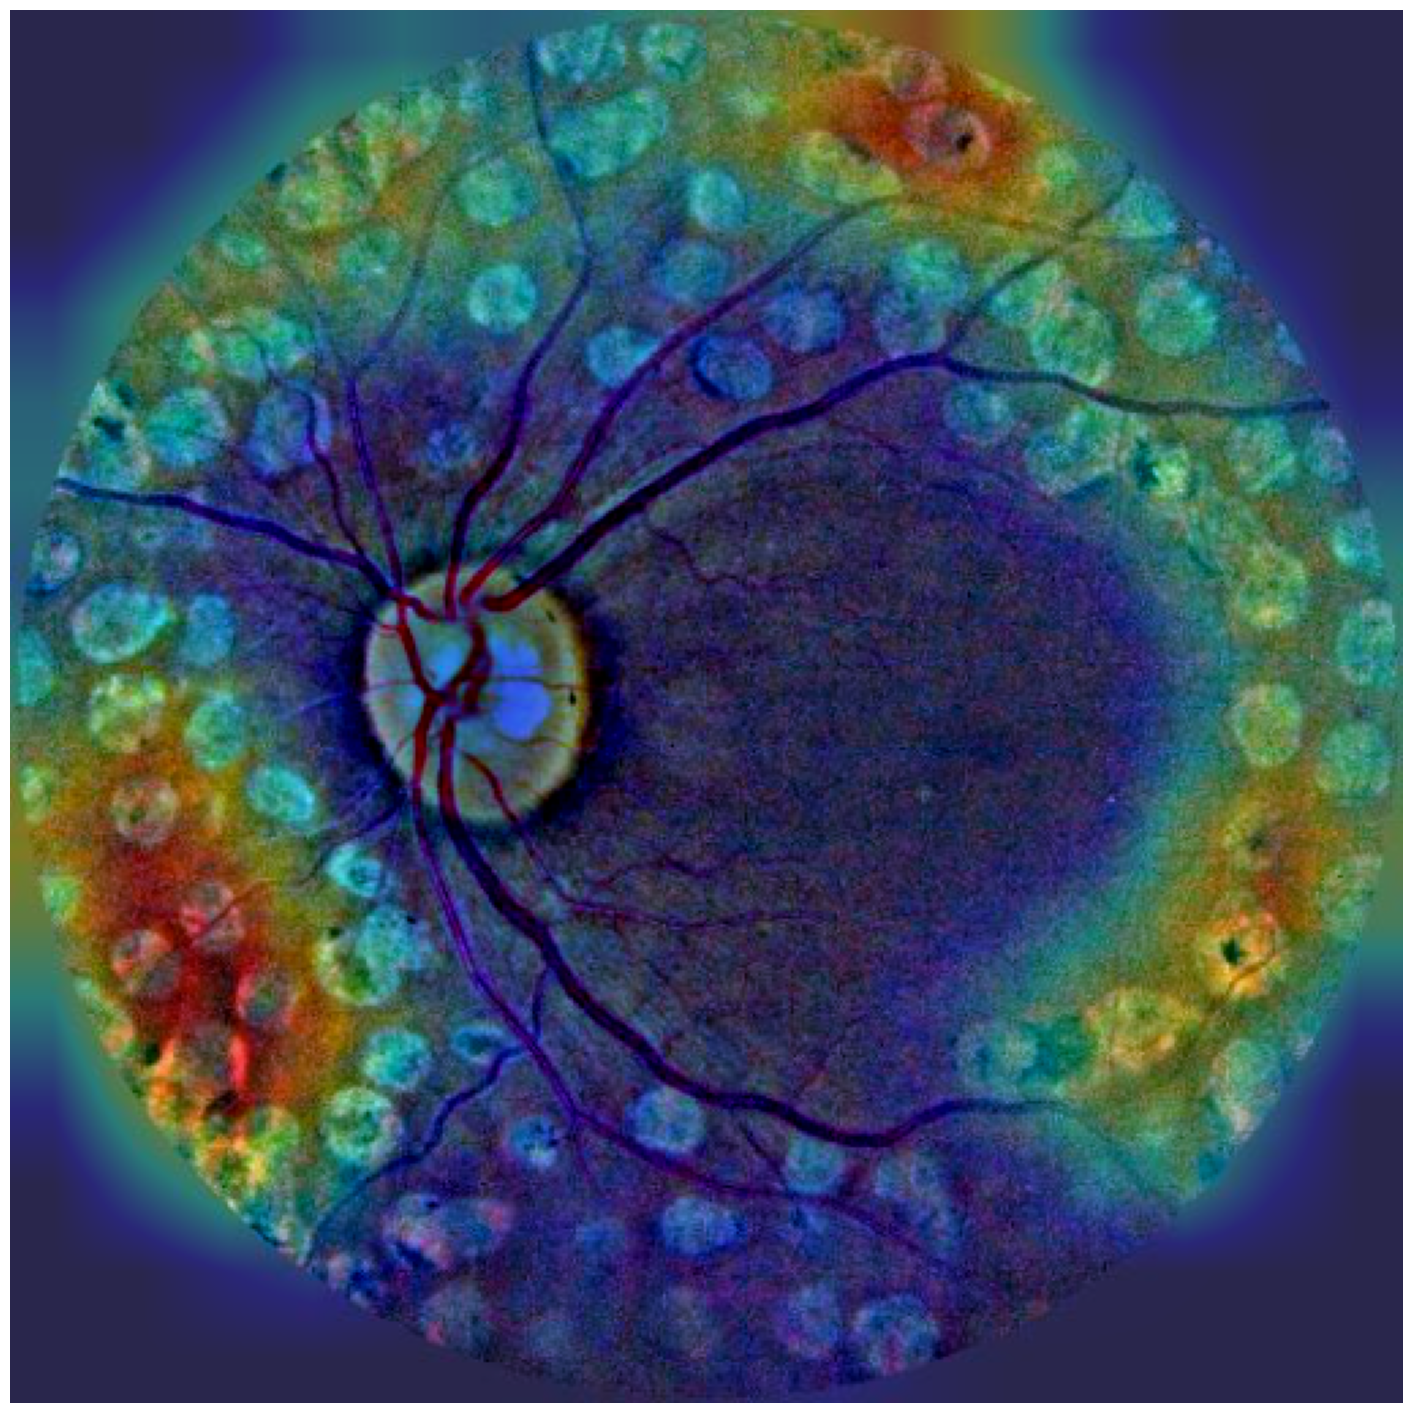
\includegraphics[width=\textwidth,height=\textwidth]{figures/chapter6/others/grad_cam4.png}
         \caption{Grad-CAM}
    \end{subfigure}
    \hfill
    \begin{subfigure}[b]{0.24\textwidth}
         \centering
         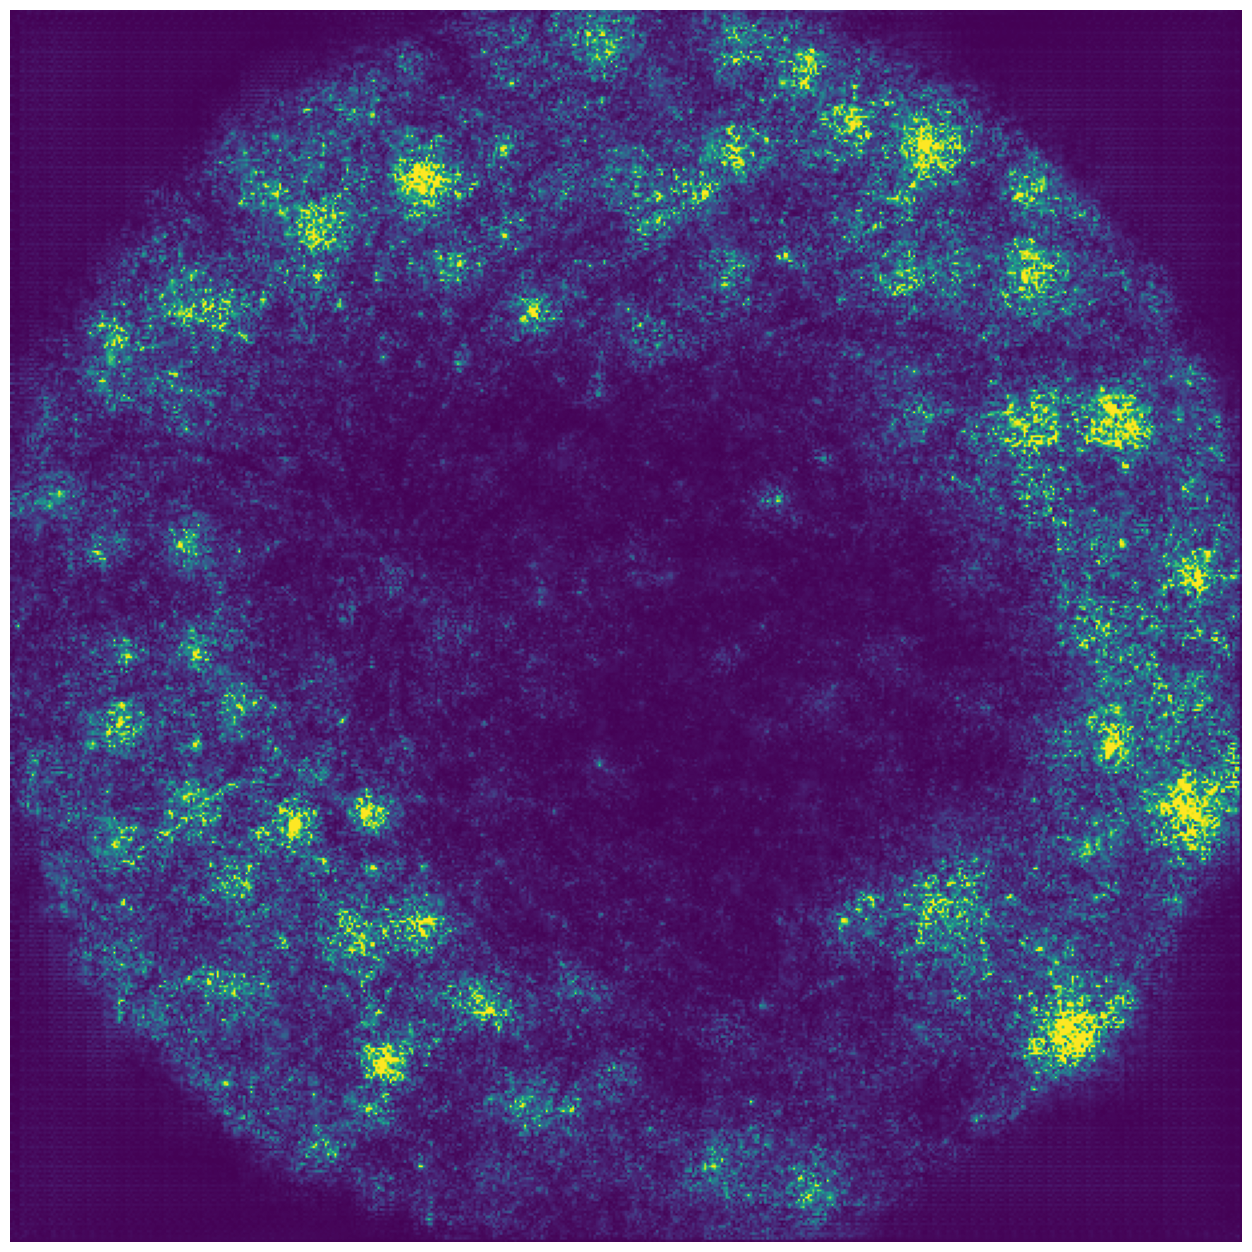
\includegraphics[width=\textwidth,height=\textwidth]{figures/chapter6/others/saliency.png}
         \caption{Saliency map}
     \end{subfigure}

     \centering
     \caption{Auxiliary visualizations for an image. Predicted: 4. Target: 4}
     \label{fig:visualizations}
\end{figure}

Guided Grad-CAM is a version of Grad-CAM that omits non-activated neurons, achieving precision at a very low level. 

Anchor maps mask those parts of the image with a low value of the CAM in order to isolate the region that is the main responsible for the classification. In the \Cref{fig:anchor}, the areas isolated by the anchor are completely covered by lesions, as we would expect for grade 4 images. 

 \textit{Saliency maps} are a more sophisticated version of Grad-CAM \cite{simonyan2013deep} that use guided gradients to obtain more precise activation maps. These visualizations can be used for other tasks; the original authors used them for weakly supervised segmentation of entities in the image. We will explore one of these uses later on, when we use feature maps to address the problem of blood vessel segmentation.

\section{Feature extraction}
We can observe the way convolutional layers work by extracting the hidden representation of the model at different steps of data processing \cite{zeiler2014visualizing}. We extracted the hidden representation of the model when the number of channels reaches certain landmarks (\Cref{fig:features}) and pooled the representation over all channels. 

\begin{figure}[tb]
    \centering
    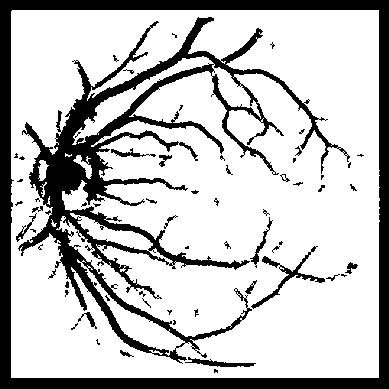
\includegraphics[scale = 0.35]{figures/chapter6/features/segmentation.png}
    \caption{Blood-vessel segmentation from features map using generic image manipulation techniques}
    \label{fig:segmentation}
\end{figure}

The extracted features can be used to debug and understand the model or fed to other models. An important utility is segmentation: recognizing the parts of the network responsible for identifying certain patterns can be used to isolate them, usually in ways that are way beyond the capabilities of generic image manipulation methods.

In this case, the inspection of the feature maps is in line with the current understanding on how convolutional neural networks work: the first layers extract low-level information as borders, middle layers extract medium-level information (as curvature or corners) and last layers synthesize very high level information \cite{zeiler2014visualizing}.

By inspecting \Cref{fig:features} we realize the model has become excellent at segmentation of blood vessels in the first convolutional layers. \Cref{fig:segmentation} shows the result of applying a threshold method with connected-components detection (from open-source ImageMagick library) to one of the features map from \Cref{fig:features}. 

Considering blood vessel segmentation is a challenging problem that requires task-specific algorithms and that the model has no pre-existing notion of blood vessels, the result shows the viability of using feature maps to address related problems. For example, segmentation of blood vessels may be used by an expert to detect vascular abnormalities that may be hard to detect in the original image.

\begin{figure}
     \begin{subfigure}[b]{0.19\textwidth}
         \centering
         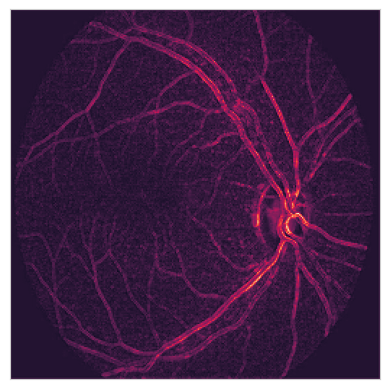
\includegraphics[width=\textwidth, height=\textwidth]{figures/chapter6/features/10988_left/10988_left_0.png}
    \end{subfigure}
    \hfill
    \begin{subfigure}[b]{0.19\textwidth}
         \centering
         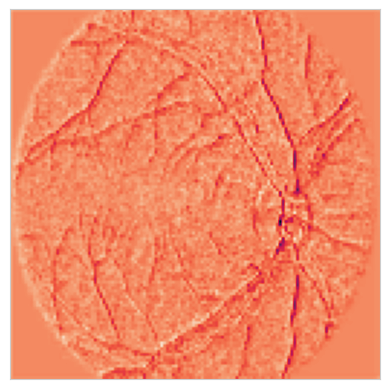
\includegraphics[width=\textwidth, height=\textwidth]{figures/chapter6/features/10988_left/10988_left_1.png}
    \end{subfigure}
    \hfill
          \begin{subfigure}[b]{0.19\textwidth}
         \centering
         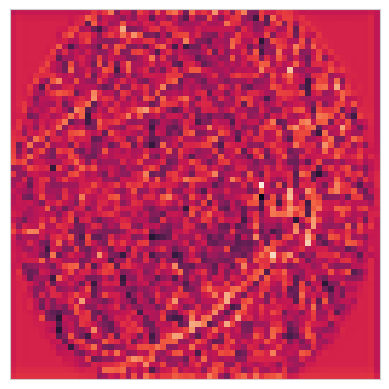
\includegraphics[width=\textwidth, height=\textwidth]{figures/chapter6/features/10988_left/10988_left_2.png}
    \end{subfigure}
    \hfill
    \begin{subfigure}[b]{0.19\textwidth}
         \centering
         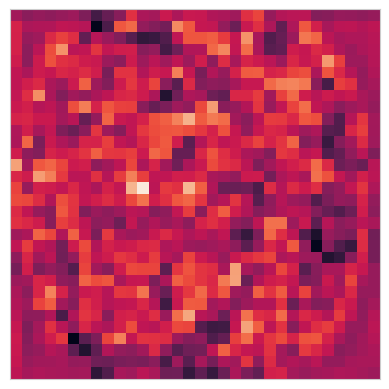
\includegraphics[width=\textwidth, height=\textwidth]{figures/chapter6/features/10988_left/10988_left_3.png}
     \end{subfigure}
     \hfill
     \begin{subfigure}[b]{0.19\textwidth}
         \centering
         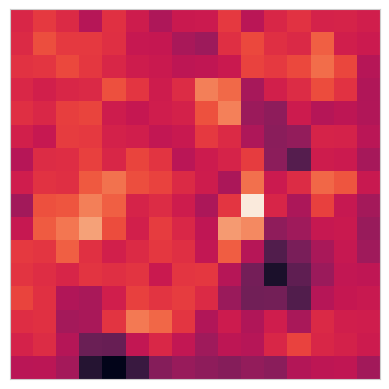
\includegraphics[width=\textwidth, height=\textwidth]{figures/chapter6/features/10988_left/10988_left_4.png}
     \end{subfigure}

    \bigskip

    \begin{subfigure}[b]{0.19\textwidth}
         \centering
         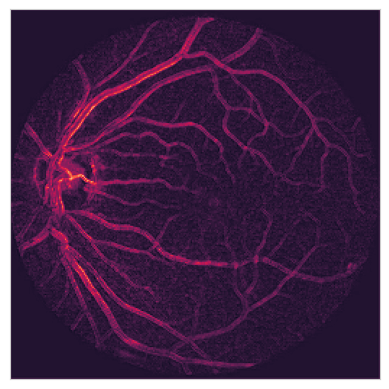
\includegraphics[width=\textwidth, height=\textwidth]{figures/chapter6/features/9521_left/9521_left_0.png}
    \end{subfigure}
    \hfill
    \begin{subfigure}[b]{0.19\textwidth}
         \centering
         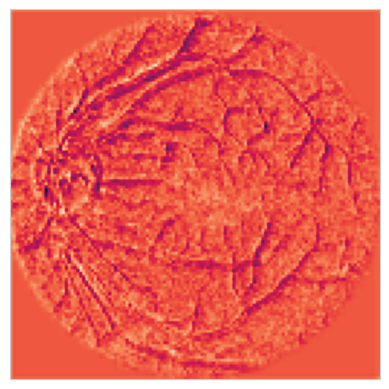
\includegraphics[width=\textwidth, height=\textwidth]{figures/chapter6/features/9521_left/9521_left_1.png}
    \end{subfigure}
    \hfill
    \begin{subfigure}[b]{0.19\textwidth}
         \centering
         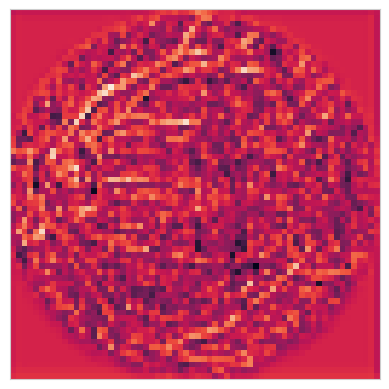
\includegraphics[width=\textwidth, height=\textwidth]{figures/chapter6/features/9521_left/9521_left_2.png}
    \end{subfigure}
    \hfill
    \begin{subfigure}[b]{0.19\textwidth}
        \centering
        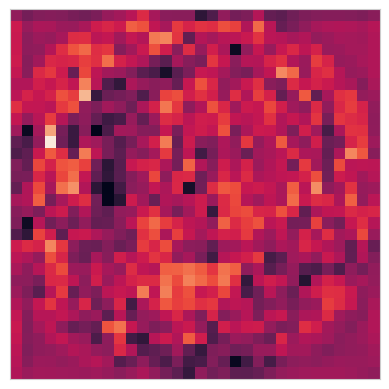
\includegraphics[width=\textwidth, height=\textwidth]{figures/chapter6/features/9521_left/9521_left_3.png}
     \end{subfigure}
     \hfill
     \begin{subfigure}[b]{0.19\textwidth}
         \centering
         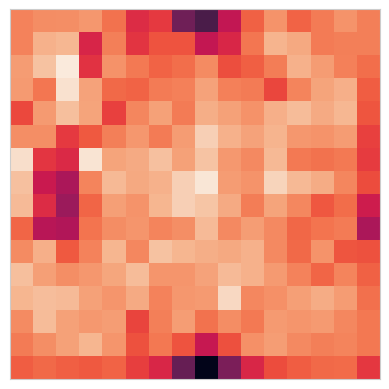
\includegraphics[width=\textwidth, height=\textwidth]{figures/chapter6/features/9521_left/9521_left_4.png}
     \end{subfigure}
     \caption{Feature maps for two images. Maps further to the right have been extracted later. The last map is the output of the convolutional block before global pooling.}
    \label{fig:features}
\end{figure}

\paragraph{Weight visualization}
If we don't pool the extracted representation, we can visualize the effect of single layers over the image across different channels. \Cref{fig:weights} shows the output of the first convolutional layer. 

\begin{figure}[tb]
    \begin{subfigure}[b]{0.49\textwidth}
        \centering
        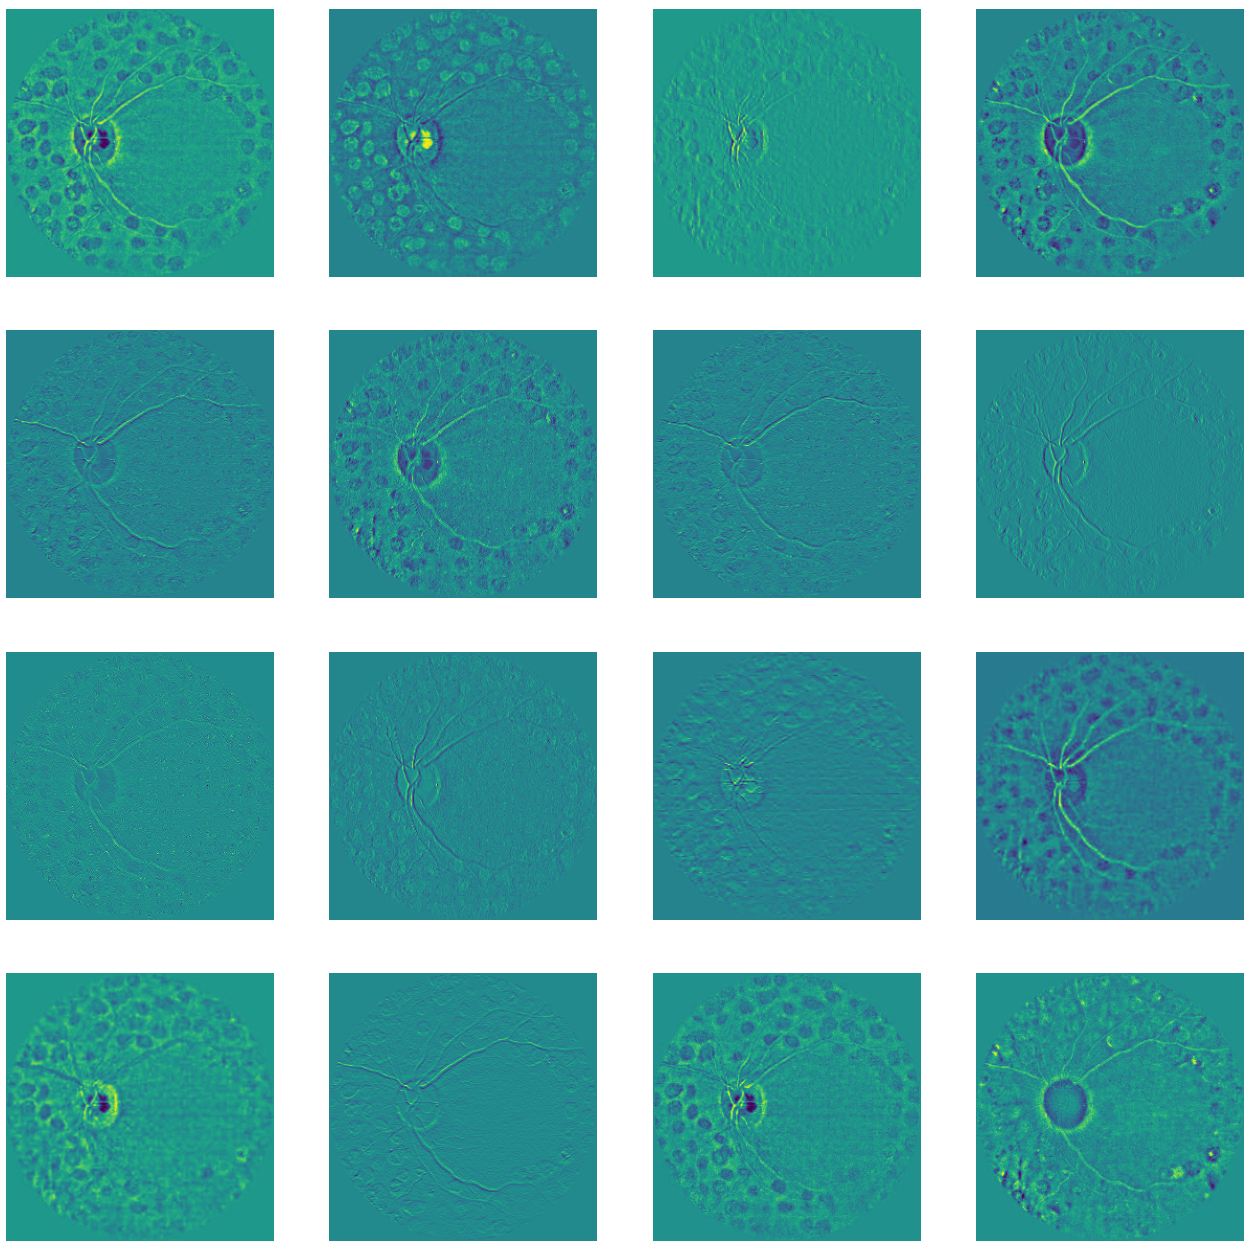
\includegraphics[height=\textwidth,width=\textwidth]{figures/chapter6/weights/kernel.png}
        \caption{First convolutional layers}
        \label{fig:weights}
     \end{subfigure}
     \hfill
     \begin{subfigure}[b]{0.49\textwidth}
         \centering
         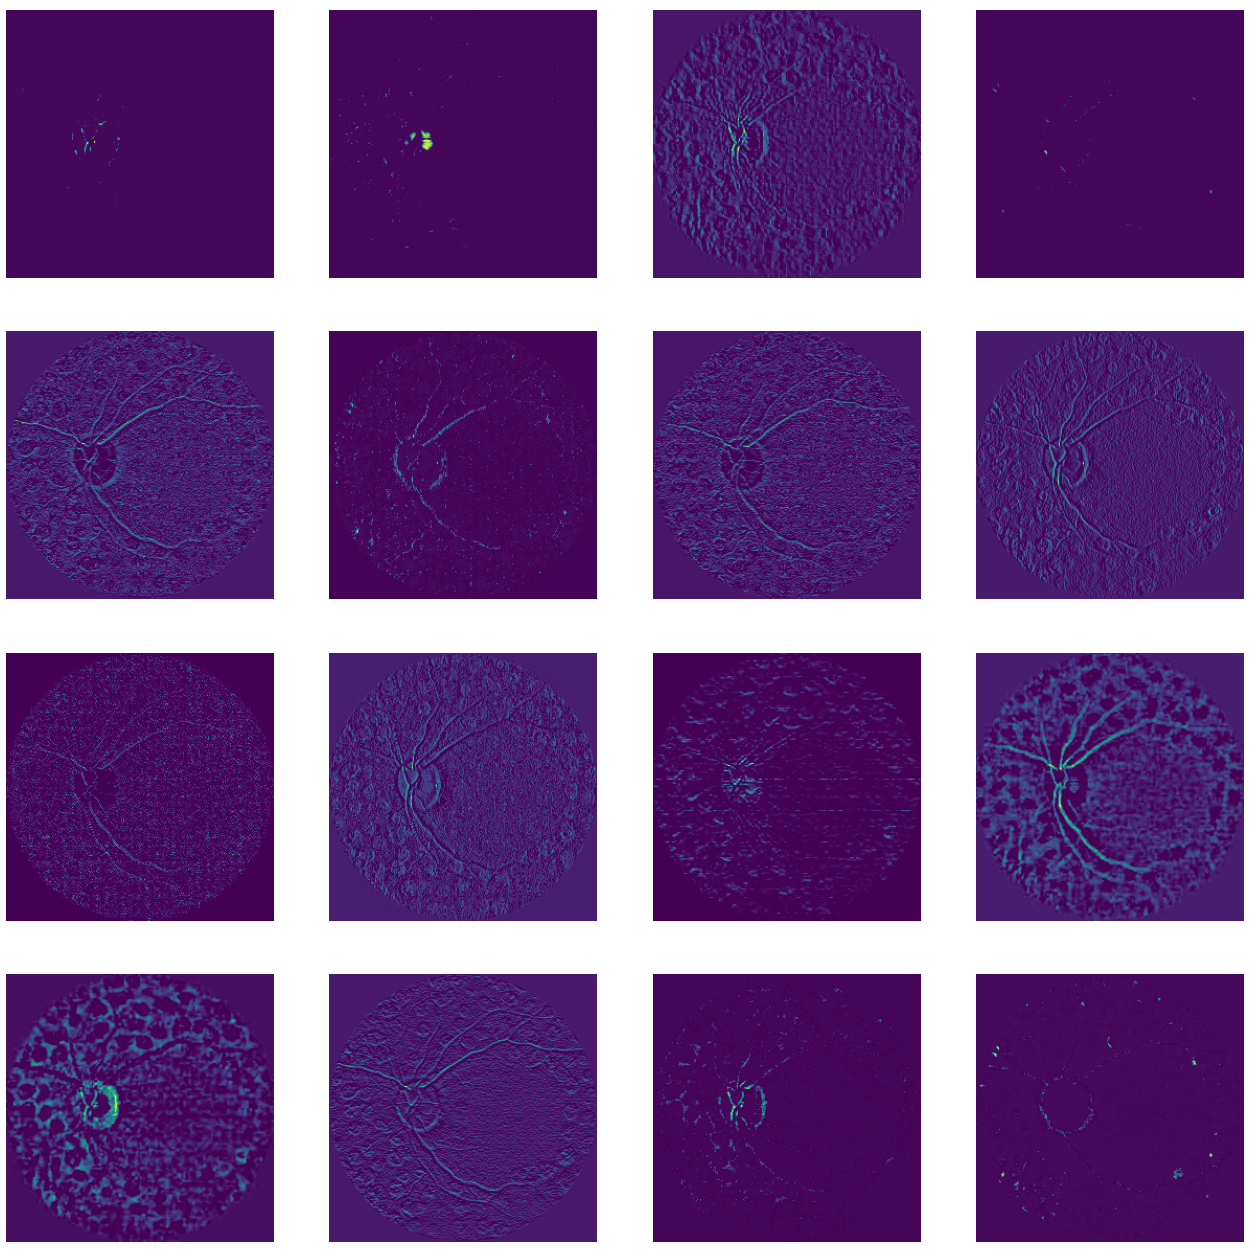
\includegraphics[height=\textwidth,width=\textwidth]{figures/chapter6/weights/maxpool.png}
        \caption{First max-pooling layer (post-activation)}
        \label{fig:activations}
     \end{subfigure}
    \caption{Output of early layers of the model. Each image represents a hidden channel. }
    \label{fig:layer_output}
\end{figure}

It is clear that some kernels are mainly responsible for extracting blood vessels, and others for extracting lesions. We observe some kernels are able to clearly segmentate the optic disk, a significant feat so early in the network.  Particularly interesting is the last filter, which recovers most of the barely visible tissue structure under the lesions.

\Cref{fig:activations} shows the effect of the first layer of max pooling and the pattern of activations. Some activations are extremely sparse, probably because they recognize very specific patterns not present in the image.
